\subsection{PyRe progress and theory}
\begin{frame}
\frametitle{PyRe: Cyclus (Py)ro (Re)processing Module}
\begin{columns}
	\begin{column}{.45\textwidth}
		\begin{block}{How does PyRe work?} 
			PyRe does the following with an input stream and facility configuration parameters: 
			\begin{itemize}
				\item Pass fuel to voloxidation.
				\item Generate efficiencies from parameters.
				\item Multiply stream by efficiency matrix.
				\item Repeated for each process.
			\end{itemize}
		\end{block}
		\begin{block}{Current Work:} 
		Create a class for each sub-process, and build the archetype. 
		\end{block}
	\end{column}
	\begin{column}{.55\textwidth}
		\begin{figure}
			\centering
			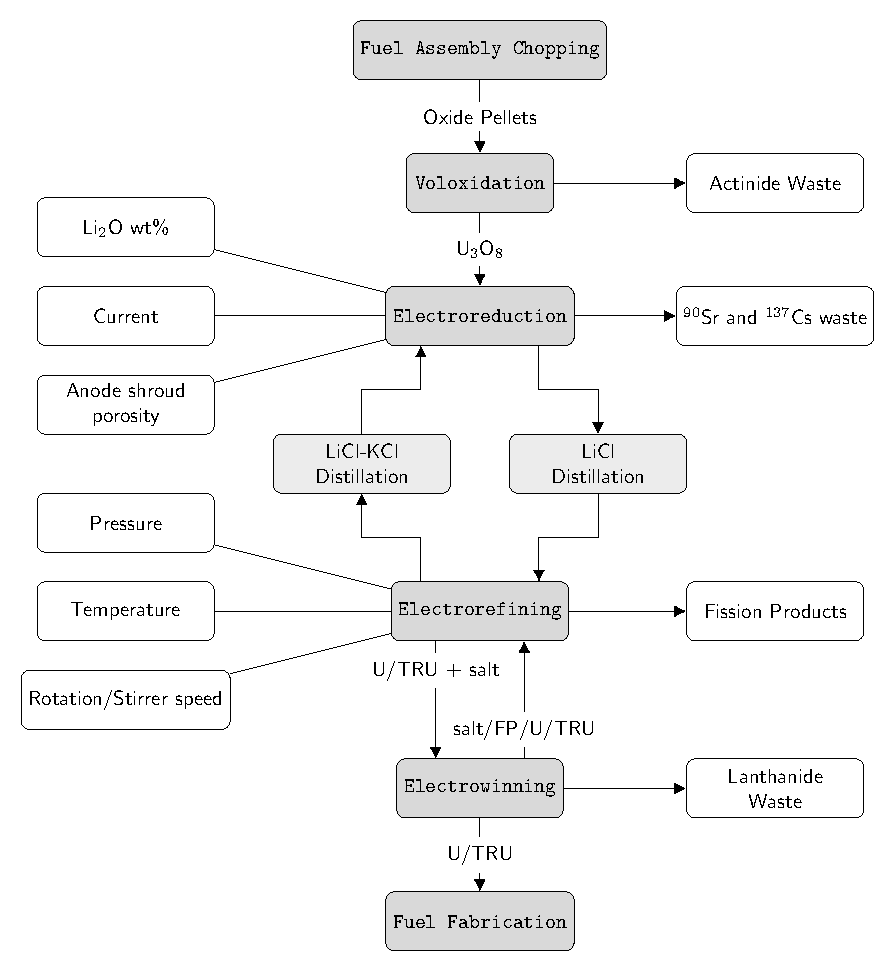
\includegraphics[width=0.9\linewidth]{flowchart}
			\caption{An archetype design flowchart of pyroprocessing facilities.}
			\label{fig:pyre}
		\end{figure}
	\end{column}
\end{columns} 
\end{frame}
\subsection{About PyRe}
\begin{frame}
\frametitle{PyRe: Cyclus (Py)ro (Re)processing Module}
\begin{block}{Timeline:} 
	The archetype will be functional with preliminary efficiencies early \textbf{August 2018}. \\
	A more detailed PyRe will be completed for ANTPC in \textbf{September 2018}.
\end{block}
\begin{block}{Archetype Uses:} 
	PyRe will answer the following questions
	\begin{itemize}
		\item What is the effect of introducing pyroprocessing plants in the fuel cycle?
		\item How do various facility designs affect throughput and efficiency?
		\item What are the best points to monitor a pyroprocessing plant for diversion?
	\end{itemize}
\end{block}
\begin{block}{Where is PyRe?} 
	PyRe can be found in the "pyre" branch of recycle: 	\href{https://github.com/arfc/recycle}{arfc/recycle.} 
\end{block}
\begin{block}{Who is working on this?}
	Greg Westphal, UIUC Graduate Researcher
\end{block}
\end{frame}

